\subsection{UART Implementation}
The UART is interrupt driven. The interrupt fires when you call
\texttt{uart\_write(uint8\_t*, int)} to signify that the buffer is non-empty by
setting a non-empty flag. There are two pointers that point to the beginning and
end of the buffer, labeled head and tail. Each character/byte is sent individually until
both the \texttt{head == tail} and the empty flag is restored. The code for the
\texttt{uart\_write} function is shown in Listing \ref{lst:uartwrite}.

\begin{lstlisting}[label={lst:uartwrite},
                   caption={UART write function and ISR}]
int uart_write(uint8_t* const str, int len){
    int overflow = 0;
    int i;

    uint8_t sreg;
    sreg = SREG;

    Disable_Interrupt();
    overflow = 0;
    for(i = 0; i < len; ++i){  
        if(non_empty && head == tail) overflow = -1;

        uart_TX_buf[tail] = str[i];

        ++tail;
        tail &= UART_TX_BUF_MASK;
    }
    
    if(overflow) head = tail;     

    if(len > 0) {

        TXIntEnable();
        non_empty = 1;
    }

    SREG = sreg;
    return overflow; 
}

/**
 * Interrupt service routine for the UART transmission.
 */
ISR(USART1_UDRE_vect) {
    UDR1 = uart_TX_buf[head];
    ++head;
    head &= UART_TX_BUF_MASK;
    // Last byte was written?
    if (head == tail){
        non_empty = 0;
        TXIntDisable();
    }
}
\end{lstlisting}

The simplest way for UART to be used is to create a character buffer and insert
the desired string using \texttt{sprinf} as shown in Listing
\ref{lst:uartwriteEx}. This makes it very simple to monitor length and insert
decimals. 

\begin{lstlisting}[float=ht,
                   caption={An example usage of \texttt{uart\_write} function},
                   label={lst:uartwriteEx}]
int len = sprintf((char *)toPrint, "X %d, Y %d\r\n", packet->x, packet->y);
uart_write((uint8_t*)toPrint, len);
\end{lstlisting}

\subsection{DC Motor Implementation}

\subsubsection{Initialization}
The D/C motor uses Pulse Width Modulation(PWM) to determine the speed at which it turns. This PWM is sent through the enable pin of the H-bridge. There is also a direction pin which must be set to either high or low.

Pin 7 on port D is set as output to be able to turn the motor on and off.
\begin{lstlisting}
 DDRD |=  (1 << PORTD7);
\end{lstlisting}

Pin 1 on port C is the direction pin, also set to output. 

\begin{lstlisting}
 DDRC |= (1 << PORTC1);
\end{lstlisting}

Finally, pin 7 on port D is the pin that outputs the PWM, also set for output. 

\begin{lstlisting}
DDRB |= (1 << PORTD7);
/** setup timer/counter 0  for fast PWM   **/ 
TCCR0A = (1 << WGM00) | (1 << WGM01) | (0 << COM0A0) | (1 << COM0A1);
TCCR0B = (0 << WGM02) | (0 << CS02) | (0 << CS01) | (1 << CS00);
\end{lstlisting}

The COM0A1/0 pins control the output of OCA0. In the motor driver, the compare output mode is set to clear OC0A when the counter matches the value in the output compare register, OCR0A, and to pull high when the counter reaches the TOP value. By setting and clearing OCA0, the pulse width that drives the motor is generated. According to the AT90USB1287 datasheet, different modes of operation will have different effect on the behavior of OC0A. The operation mode we are using is Fast PWM mode. It can be set by setting WGM02/1/0 to 011. The last thing that the motor initialization function does to set the clock prescaler. CS02/1/0 determines the prescale factor. For us, we set CS02..0 to 001 which disables the prescaling.

\begin{figure}[tbp]
  \begin{center}
    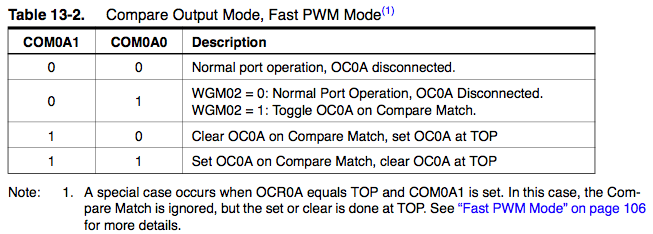
\includegraphics[width=125mm]{imageSources/pwmTable1.png}
  \end{center}
  \caption{Fast PWM Mode} 
  \label{pwmTable1}
\end{figure}

The above table outlines the 8 different types of  Waveform generation that are available. As can be seen by how we set the code, we chose to use mode7. This describes that the system uses fast PWM and that the top value is defined by OCRA.  As can be seen in the following section, we change the value of OCR0A to  change the speed of the motor.

\begin{figure}[ht]
  \begin{center}
    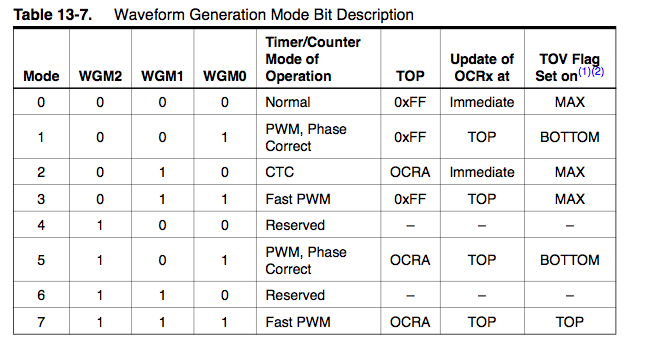
\includegraphics[width=125mm]{imageSources/waveformGenerationTable.png}
  \end{center}
  \caption{Waveform Generation Mode Bit Description} 
  \label{waveformGenerationTable}
\end{figure}

\subsubsection{Control}
To control the speed of the D/C motor, we use the function called setMotorSpeed(uint8\_t). The duty parameter sets the duty cycle period of the pulse. The larger the duty cycle is, the faster the motor will spin. 

\begin{lstlisting}
 void setMotorSpeed(uint8_t duty) {
	OCR0A = duty;
}
\end{lstlisting}

Aside from the speed of the D/C motor, we need to have control of the direction of which the motor will spin. In the motor driver code, there is a function called, setMotorDirection(int), which can be used to set the direction. 

\begin{lstlisting}
void setMotorDirection(int d) {
    if (d == BACKWARD)
        PORTC |= _BV(PORTC1);
    else
        PORTC &= ~(_BV(PORTC1));
}
\end{lstlisting}

This code will either set the C1 pin High or Low. By doing this, the switches changes the direction pin on the H-bridge. See the explanation of H-Bridge in the Hovercraft Design and Construction section. 

\subsection{Joystick Implementation}
The joystick is sampled every second. The x, y, and z values of the joystick are sent by the radio from the base station to the hovercraft. On the hovercraft end, it will translate those x, y, and z values into speed/direction of the motor as well as the the degree of which the servo motor should turn. The x, y, and z values from the joystick is converted into digital signals by using the analog to digital converter (ADC) built into the AT90USB1287. Please refer to the joystick section of Hardware Overview.

\subsubsection{Analog-to-Digital Conversion}
To start a conversion from an analog signal to a digital signal, both ADEN (bit 7) and ADSC (bit 6) need to be set in the ADC Control and Status Register A (ADCSRA). As shown in the following code snippet.
\begin{lstlisting}
#define TAKE_SAMP (_BV(ADEN) | _BV(ADSC))
ADCSRA = TAKE_SAMP;
\end{lstlisting}

Since there are three inputs (x, y, and z) from the joystick,  the ADC multiplexer(ADMUX) is used to select which input value for the ADC to sample.

\begin{lstlisting}
// X value
#define SAMP0 	(_BV(REFS0) | _BV(ADLAR) | PINF1)
// Y value
#define SAMP1 	(_BV(REFS0) | _BV(ADLAR) | PINF2)
// Z value
#define SAMP2 	(_BV(REFS0) | _BV(ADLAR) | PINF4)
\end{lstlisting}

The bit ADSC is also used to determine if a conversion is in progress. It will stay high as long as there is an ongoing conversion; as soon as the conversion is completed it will become low. The following function demonstration how to use the ADSC to determine when to read the ADC results from the ADCH register. The result of the conversion can be found in the ADC Result Register (ADCL, ADCH) which is a 16-bit register. If the ADLAR bit in ADMUX register is set to high, the result is left adjusted, which means one can read the result from ADCH. If, however, the ADLAR bit is low, the result is right adjusted, so the result will be stored in ADCL.

\begin{lstlisting}[float=ht]
#define ADC_NOT_DONE() 	(ADCSRA & _BV(ADSC)) 
static void single_sample(unsigned char SAMPN, int input_num) {
	ADMUX = SAMPN;
	//need to sample multiple times, because A/D seems to have some
	//memory of the previous value that was read

	ADCSRA = TAKE_SAMP;
	while (ADC_NOT_DONE()){}
	ADCSRA = TAKE_SAMP;
	while (ADC_NOT_DONE()){}
	ADCSRA = TAKE_SAMP;
	while (ADC_NOT_DONE()){}

	sum[input_num] = ADCH;
}
\end{lstlisting}

\subsection{Servo Implementation}
Similar to the DC motor, the servo motor is controlled by pulse width modulation (PWM). Initializing the servo driver is very similar to the DC motor initialization function. First, a clock prescaler is chosen by setting the CS02/1/0 bits in TCCR1B. In the servo driver code, CS02/1/0 is set to 010 which sets the prescale factor to 8 or the clock is running at 1Mhz. Also we set the waveform generation mode to fast PWM mode by setting WGM13..0 to 1110. As for the output to the servo, we configure the OC1B pin to go high when the timer/counter is equal to OCR1B (= 800), and OC1B pin to go low when the timer/counter equals to ICR1 (=20000). Such configuration is done through setting COM1B1..0 pins to 10.

\begin{lstlisting}
void
servoInit(void){

	TCCR1B = (0 << CS10)|(1 << CS11)|(0 << CS12)|(1 << WGM13)|(1 << WGM12);

	TCCR1A = (0 << WGM10) | (1 << WGM11) | (1 << COM1B1) | (0 << COM1B0);
	/*Set the IO pins for output for  OCB1*/
	DDRB = 0xFF;
	/* Set the TOP value to 2500 this should mean that the TCNT1 counter
	 should reset itself every 50 Hz at a clock of 1Mz for 8 Mhz, set to 20000(hopefully)*/
	ICR1 = 20000;
	/* Set the low timings for the three output pins for ports A in OCR1A*/
	OCR1B = 800; //corresponds to 8% duty cycle or 2ms pulse width
}
\end{lstlisting}

After initialization and configuration, the servo can be easily controlled by setting the OCR1B register.

\begin{lstlisting}
int servoDuty(int duty){
	OCR1B = duty;
	return duty;
}
\end{lstlisting}

\subsection{Sonar Implementation}
There are two stages when it comes to how the sonar operates. The first stage, the sonar sends out seven 42Khz pulses. Then, the second stage, is to the use the echoes and the PW pin on the sonar to get a pulse width representation of range. Aside from using the pulse width representation, MaxSonar can also use the TX pin to asynchronous deliver range information in RS232 format. There is another option available to acquire range data from the MaxSonar---using the ADC built into the AT90USB; the AN pin on the MaxSonar will output 0 to 2.55 volts with a factor of 10mV per inch

The sonar driver we are using uses the pulse width method. In the pulse width method, the duration of the duty cycle is used to determine the range. According the datasheet 1 inch is equal to 147uS. Since the duration is the key factor in order to determine the range, an input capture unit is used to determine the time of which the signal is pulled high as well as the time of which the signal goes low. Once the two timestamps are known, we can calculate the difference, determine the duration and range. The input capture unit is found in one of the 16-bit timers (we are using timer 3). Hence the initialization is pretty similar to other peripherals aforementioned.

\subsubsection{Initialization}
The first initialization step is to set the clock source and choose a clock prescaler. The clock prescale factor is chosen by setting CS32/0 bits in the Timer/Counter3 Control Register (TCCR3B) to 010 which translates to the system clock speed divided by 8 (=1Mhz). After the clock source is set, we choose to enable the noise canceler by setting the ICNC3 bit in TCCR3B. Enabling the noise canceler allows for more reliable range data with the cost of four system clock cycles of delay, because the canceler will take four samples, and all of those four samples have to be of equal value before the change is propagated to the edge detector which might then triggers an interrupt. In order to get notified about the incoming range information from the sonar, the input capture interrupt is used. First, we need to determine which edge on the Input Capture Pin (ICP3) will trigger an event. When an event is triggered the counter value will be stored in the Input Capture Register 3 (ICR3) and the corresponding Input Capture Flag 3 (ICF3) bit is set. The ICF3 bit may then optionally cause an interrupt to fire, only if the input capture interrupt is enabled. In the initialization code, an event is set to trigger whenever a rising edge is detected. This is done by setting the ICES3 bit in TCCR3B register to high. Next, the input capture interrupt is enabled as well as the ICF3 bit in the Timer/Counter3 Interrupt Flag Register 3 (TIFR3) is cleared (Note: ICF3 bit is cleared by writing a logic one to its bit location). The last thing the initialization code does is to let the sonar performs a calibration cycle by setting the RX pin (PINC7) high.

\begin{lstlisting}
#define SONAR_PORT      PORTC
#define SONAR_ECHO_MASK (_BV(7))                                        
void sonar_init(){
//      initialize sonar
	DDRC |= _BV(7);                       
    TCCR3B &= ~(_BV(CS32) | _BV(CS30));     
    TCCR3B |= _BV(CS31);                            
    TCCR3B |= _BV(ICNC3);                           
//      enable timer and global interrupts
    TCCR3B |= _BV(ICES3);
    TIFR3  |= _BV(ICF3);
    TIMSK3 |= _BV(ICIE3);
    PORTC |= _BV(7);
    sei();
	int i=0;
    for(i=0; i < 63; ++i) _delay_ms(40);
}
\end{lstlisting}

\subsubsection{Range Calculation}
The majority of the calculation is done through the input capture interrupt. The ISR will determine what triggers the event. If it is an rising edge that triggers the event, it will set the set the counter to 0. Then the behaviour of the input capture interrupt is changed so that the interrupt will fire on a falling edge. In order to change the input capture interrupt behaviour the ISR sets the ICES3 bit to 0. After updating the interrupt firing behaviour, the input capture flag is cleared. According to the AT90USB1287 data sheet, the ICF3 bit must be cleared every time an edge changes (Again, ICF3 is cleared by writing a logical one to the corresponding bit location). After a rising edge is detected, the timer/counter is to set to 0 and the interrupt is configured to fire when a falling edge is detected. If a falling edge occurs, the timestamp will saved to the ICR3 register. In the ISR, when the triggering event is a falling edge event, the timestamp is read from ICR3 and stored to a global variable called, time\_falling, which essentially is the duration of the duty cycle. Then the input capture interrupt is changed back to detect a rising edge.

\begin{lstlisting}
#define IS_RISING_EDGE()   (TCCR3B & _BV(ICES3))
#define IS_FALLING_EDGE()  ~(TCCR3B & _BV(ICES3))
#define SET_RISING_EDGE()  (TCCR3B |= _BV(ICES3))                          
#define SET_FALLING_EDGE() (TCCR3B &= ~(_BV(ICES3)))                       
#define CLEAR_IC_FLAG()    (TIFR3 |= _BV(ICF3))
ISR(TIMER3_CAPT_vect) {
	DISABLE_PULSE();                                        
	recieved = 1;
	if (IS_RISING_EDGE()) {
		TCNT3=0;
		SET_FALLING_EDGE();
		CLEAR_IC_FLAG();
	} else {
		time_falling = ICR3;                    
		SET_RISING_EDGE();
		CLEAR_IC_FLAG();
	}	
}
\end{lstlisting}

Finally, the actual distance can be calculated by dividing the duration of the duty cycle by 147 (which is given by the MaxSonar datasheet). The result will be the distance in inches.

\begin{lstlisting}
#define US_PER_INCH 147
uint8_t read_distance() {
	return (time_falling/US_PER_INCH);      
}
\end{lstlisting}

\subsection{Radio Implementation}
The radio driver the team chose was quite straightforward to use, but it takes a lot of testing when it comes to fully configuring the radio. Before using the radio driver, one has to determine the addresses and the channel to be used by the base station and the hovercraft. For the base station, the address 0xDEAD was used, and for the hover station, the address 0xFACE is used. The radio units will be operating on channel 115.

\subsubsection{Radio Modes}
The TRW-24G radio unit used has three primary modes and a few sub-modes. Those primary modes as well as the pin settings for changing into a particular mode is listed below.

\begin{figure}[tpb]
  \begin{center}
    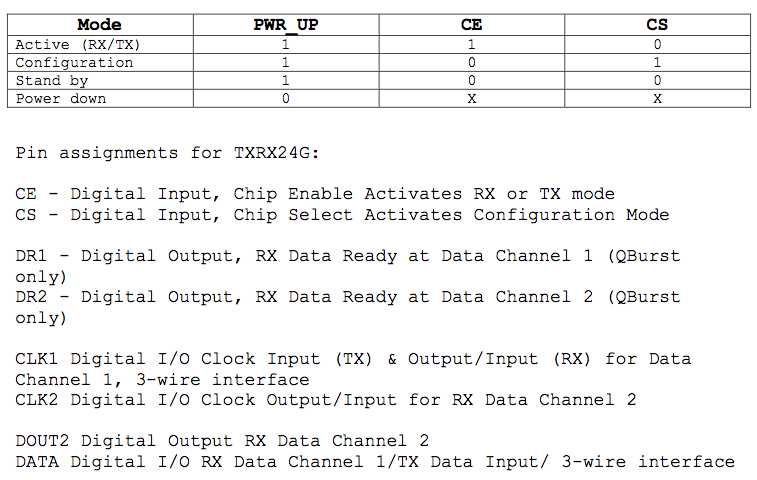
\includegraphics[width=125mm]{imageSources/radioModes.png}
  \end{center}
  \caption{Radio Modes} 
  \label{radioModes}
\end{figure}

\subsubsection{Radio Initialization and Configuration}
Before the radio can be used to transmit data, it has to be configured. The configuration involves setting the radio address, setting the operation mode (receive mode or transmit mode), as well as other configurations which can be found in the radio's datasheet. In total, the configuration word can be up to 15 bytes long. An overview of the configuration is shown below.

\begin{figure}[htp]
  \begin{center}
    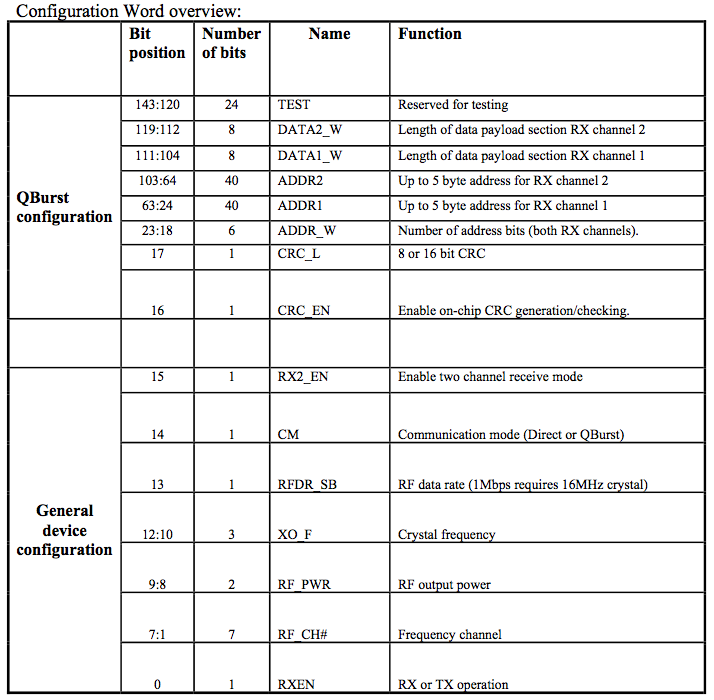
\includegraphics[width=125mm]{imageSources/radioConfigOverview.png}
  \end{center}
  \caption{Radio: Word Configuration Overview} 
  \label{radioConfigOverview}
\end{figure}

The majority of the radio initialization code is to deal with the configuration of the radio, but at the end of the radio\_init function, INT4 is enabled such whenever a packet arrives, the ISR can handle it.

\begin{lstlisting}
int radio_init(uint16_t address, uint8_t rx_enable)
{
   // ...
   // For brevity most of configuration code is cut out.
   set_rxtx_mode();

   /* Enable external interrupt on INT4 when in RX mode */
   if (rx_enable)
   {
      EIMSK |= _BV(INT4);
   }
   return 0;
}
\end{lstlisting}

\subsubsection{Sending and Receiving}
The radio driver relies on interrupt 4 (INT4) to receive packets and for sending packets, the radio must switch to transmit (if it isn't already), then the function \texttt{radio\_send()} can be used to send out packets. In the INT4's ISR, the packet is read one byte at a time into a buffer, then the buffer can be interpreted in any way you see fit. Since TRW24G is a half-duplex radio, the radio must be set to receive mode before it can receive any packets, and vice versa for the sending out packets.

\begin{lstlisting}[float=ht, 
                   caption={Radio Modes}]
void radio_set_transmit(void) {
   set_config_mode();
   put_byte(RADIO_CHANNEL << 1);
   set_standby_mode();

   /* Set DATA pin to output */
   DATA_DDR |= _BV(DATA_PINNUM);

   /* Disable external interrupt on INT4 */
   EIMSK &= ~(_BV(INT4));

   set_rxtx_mode();
} 

void radio_set_receive(void) {
   int i;
   set_config_mode();
   put_byte((RADIO_CHANNEL << 1) | 0x1);
   set_standby_mode();

   /* Set DATA pin to input */
   DATA_DDR &= ~_BV(DATA_PINNUM);

   /* Enable external interrupt on INT4 */
   EIMSK |= _BV(INT4);

   set_rxtx_mode();

   for (i=0; i<250; ++i) {
      delay_1us(); // Tsby2rx = 202 us
   }
}
\end{lstlisting}

The radio mode is set through the configuration word mentioned in the
configuration section. The key bit is the 0 bit of the first byte of
configuration word. When the 0 bit is set to 1, then the radio is receive and if
the 0 bit is 0 the radio will operate in transmit mode.

Due to a bug in the radio driver, the \texttt{radio\_set\_receive()} function
must be called twice in order to switch the radio into receive mode.  Fail to do
so may leave the whole system in an unknown and inoperable state.

\subsection{Communication Protocol}
As a part of the requirement for the team, two hovercrafts are to be built, and
there has to be interactions between the two hovercrafts. The two hovercrafts
have a master-slave relationship. The communication of
the hovercrafts is done through the radio. Please refer to section
\ref{radioconn} for details about the radio units that the hovercrafts
are using. In this project, one of the hovercrafts will be the leader, and
it is responsible for sending movements packets to the trailing hovercraft. To
facilitate the communication, a protocol is in place between the two
hovercrafts. The leader (or leading hovercraft) is also responsible for
navigating the environment, deciding what movements to use to traverse the
environment, and relaying those movements to the trailing hovercraft.

The protocol structure is shown in Figure \ref{fig:protocol}. The leader will
start navigating the environment when the base station sends an
\texttt{initiate} message. After the leader receives the \texttt{initiate}
message, it will attempt to contact the trailing hovercraft. The leader detects
the trailing hovercraft by sending a \texttt{ping} message to the trailing
hovercraft. When the trailing hovercraft receives the \texttt{ping} message, it
will response with a \texttt{pong} message. When the leader receives the
\texttt{pong} message, it will start the sensors sampling process. At the same
time, the leader will continuously send its status, as well as, sensors
information back to the base station. When the leader makes a decision about
the movement, it will relay the motors' speeds to the trailing hovercraft. If
the trailing hovercraft receives the motors' speeds information, it will
acknowledge the information back to the leaders. In order to make the process a
little more robust, there is a timeout in place in the leader. When the leader
does not receive the acknowledgments from the trailing hovercraft, it will
resend the motors speeds information again. After three timeouts, the leader
will give up and continue on its way.
\begin{figure}[thp]
  \begin{center}
    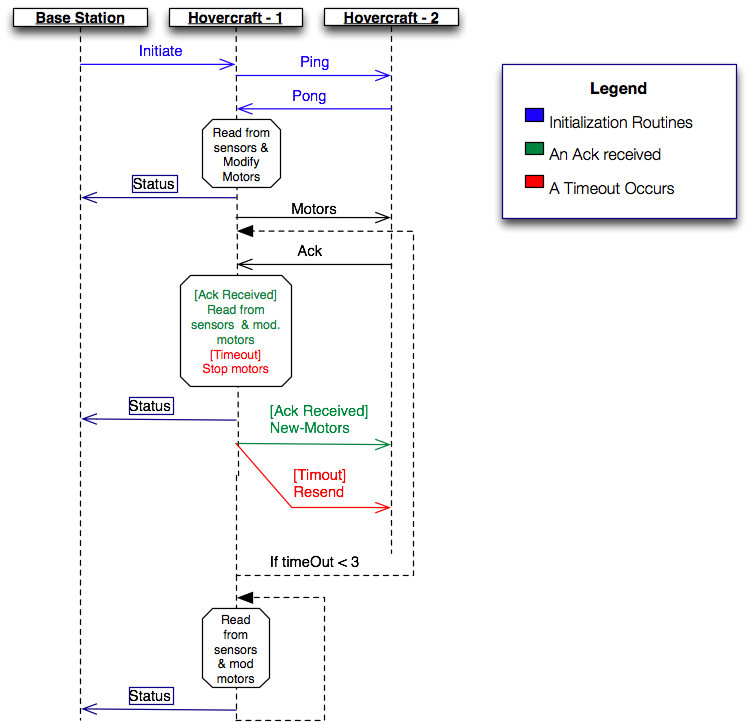
\includegraphics[width=130mm]{imageSources/messages.png}
  \end{center}
  \caption{Protocol Structure Between the Hovercrafts} 
  \label{fig:protocol}
\end{figure}

\subsubsection{Protocol Implementation}
In terms of the implementation, all those messages in Figure \ref{fig:protocol}
are represented as C structures. First there is a \texttt{enum} type that is
used to represent the different types of messages. The \texttt{enum} type is
shown in listing \ref{lst:msgenum}.
\begin{lstlisting}[caption={Enumerations for message types},
                   label=lst:msgenum]
typedef enum { INIT=1, PING, PONG, INFO, MOVE, ACK } packet_t;
\end{lstlisting}
There is a generic structure with only one field. This generic structure is used
to determine the actual type of the message. Since the radio units that the
hovercrafts are using, send an array of bytes. There needs to be a way to figure
which message type those bytes belong to. The definition of the generic
structure is shown in Listing \ref{lst:generic} and the code that is used to
determine the type of the message is shown in Listing \ref{lst:genericusage}. In
Listing \ref{lst:genericusage}, the bytes received from the radio is, first,
cast to the generic packet type, then a \texttt{switch} statement is used to
determine the actual message type.
\begin{lstlisting}[label=lst:generic,float,
                   caption={Generic Packet Structure}]
typedef struct genericPacket {
    packet_t type;
} genericPacket_t;
\end{lstlisting}
\begin{lstlisting}[label=lst:genericusage,float,
                   caption={Packets Casting}]
ISR (INT4_vect) {
    int i;
    PORTD ^= _BV(PORTD5);
    for (i = 0; i < PAYLOAD_BYTES; i++) {
        radio_buffer[i] = radio_get_byte();
    }
    
    // Figure out what type of packet this is.
    genericPacket_t *incomingPacket = (genericPacket_t *)radio_buffer;
    movePacket_t *theMovePacket;
    switch(incomingPacket->type) {
        case PING:
            pingReceived = true;
            break;
        case MOVE:
            theMovePacket = (movePacket_t *) radio_buffer;
            rightMotorSpeed = theMovePacket->rightMotor;
            leftMotorSpeed  = theMovePacket->leftMotor;
            needSendAck = true;
            break;
        default:
            // ignore
            break;
    }
    
    /* setup the radio to receive another packet */
    radio_set_receive();
}
\end{lstlisting}
The rest of the definition for the different types of messages is listed in
Listing \ref{lst:mesgtypes}.
\begin{lstlisting}[label=lst:mesgtypes,float,
                   caption={Message Types Definitions}]
typedef struct initPacket  {
    packet_t type;
    uint8_t init:1;
} initPacket_t;

typedef struct pingPacket {
    packet_t type;
    uint8_t ping:1;
} pingPacket_t;

typedef struct pongPacket {
    packet_t type;
    uint8_t pong:1;
} pongPacket_t;

struct infoPacket {
    packet_t type;
    uint8_t resend:1;
    uint8_t frontSonar;
    uint8_t rightSonar;
    uint8_t leftSonar;
    uint8_t rightMotor;
    uint8_t leftMotor;
};

typedef struct movePacket {
    packet_t type;
    uint8_t rightMotor;
    uint8_t leftMotor;
    direction_t rightDirection;
    direction_t leftDirection;
} movePacket_t;

typedef struct ackPacket {
    packet_t type;
    uint8_t ack:1;
} ackPacket_t;

struct resendPacket {
    packet_t type;
};
\end{lstlisting}

